\chapter{Analysis Models}
\label{chap:AM}

%This chapter provides a general overview of the main concepts gathered during
%the analysis phase, in particular those concerning the software system types
%(i.e. classes, datatypes, and enumerations), as well as the actors that
% interact with the software system through their interfaces. Figures included in the
%Messir Requirement Document that correspond to the  the \glspl{Concept Model}
% and the \glspl{Environment Model} could be also included in this chapter, as a means of synthesizing what
%are the requirements to which the design is supposed to sketch a solution.


\section{Flow-orineted model}
This model provides an indication of how data objects are transformed by a set
of processing functions.

\begin{figure}[h]
	\centering	
	\captionsetup{justification=centering}
	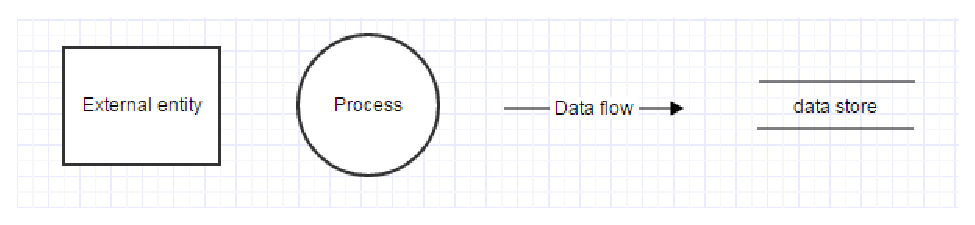
\includegraphics[width=0.5\textwidth]{./images/flow_notation.eps}
	\caption{Data Flow notation}
\end{figure}


\begin{figure}[h]
	\centering
	\captionsetup{justification=centering}
	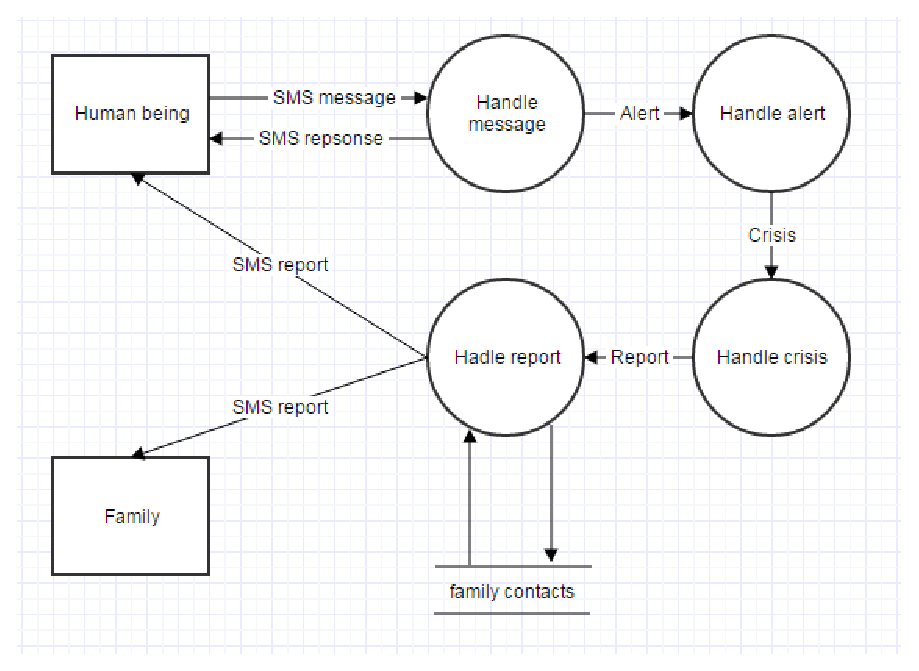
\includegraphics[width=0.5\textwidth]{./images/data_flow_diagram.eps}
	\caption{Data Flow diagram}
\end{figure} 

\section{Csenario-based model}
This model represents the system from the user's point of view.

\subsection{Use Cases}

\subsubsection{summary-suDeployAndRun}

The goal is to install the iCrash system on its infrastructure and to exploit its capacities related to the
secure administration and eficient handling of car crash situations depending on
alerts received.


\begin{figure}[h]
	\centering	
	\captionsetup{justification=centering}
	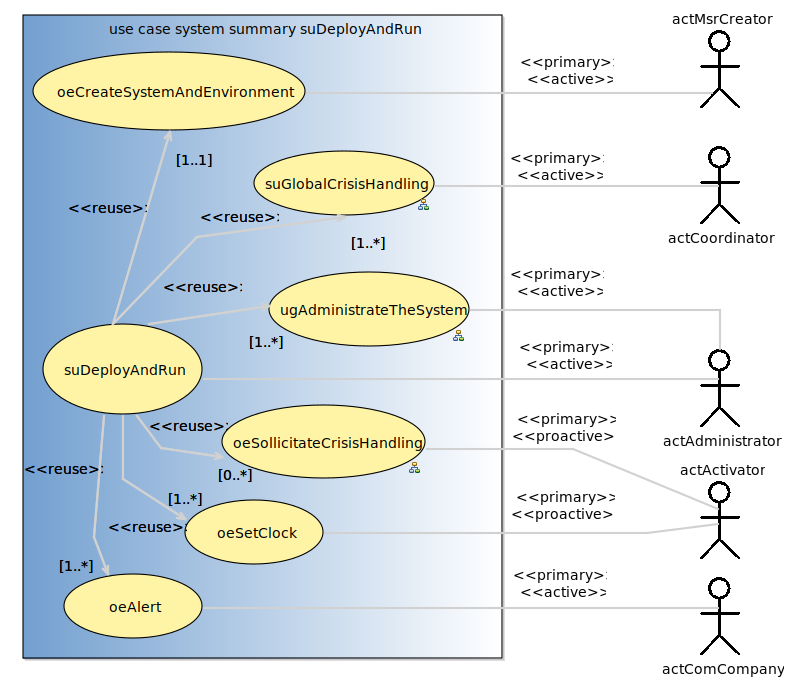
\includegraphics[width=0.5\textwidth]{./images/uc-suDeployAndRun.eps}
	\caption{Use case diagram for the suDeployAndRun summary use case}
\end{figure}


\section{Concept Model}
 

\begin{figure}[h]
	\centering
	\captionsetup{justification=centering}
	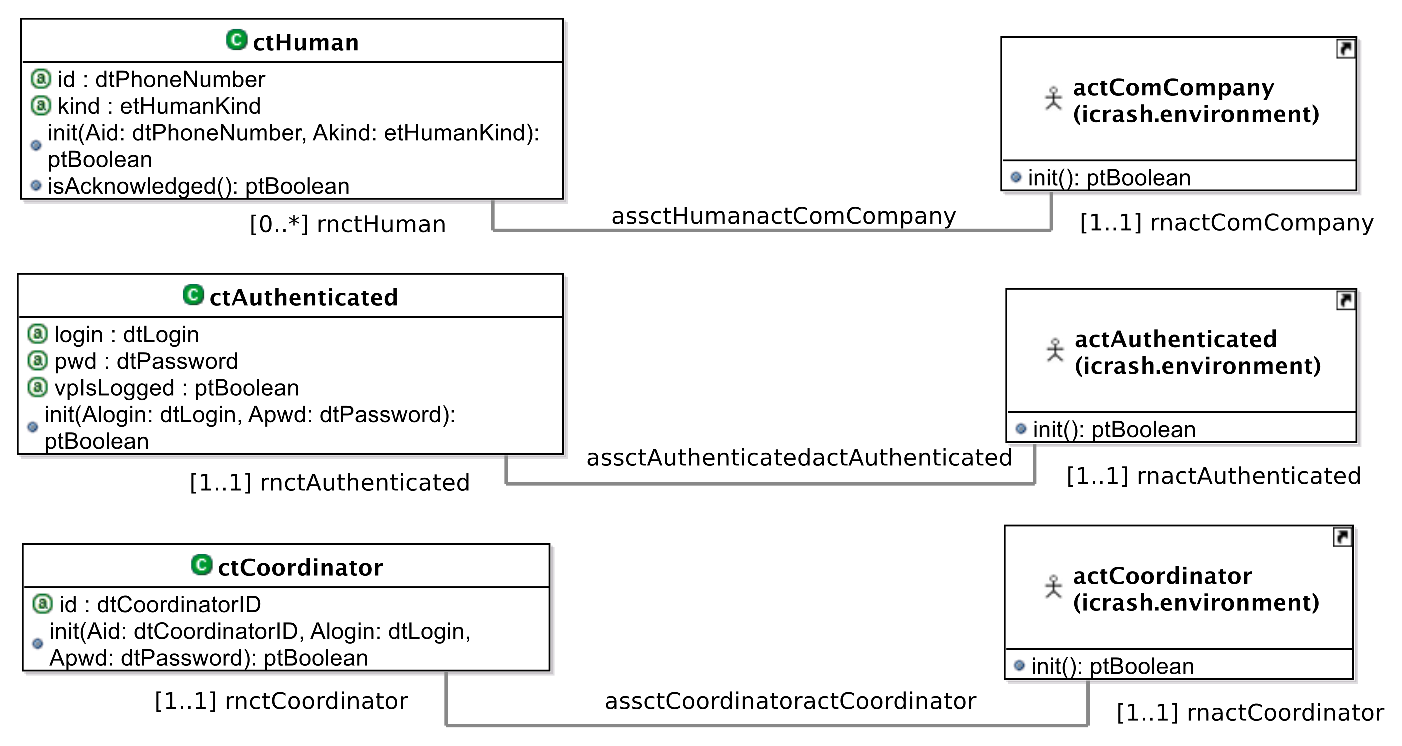
\includegraphics[width=0.5\textwidth]{./images/analysis/concept-model/global/PrimaryTypes-Classes/01/cm-pt-ct-gv-01.eps}
	\caption{--}
\end{figure} 


   

\section{Environment Model}

\begin{figure}[h]
\begin{center}
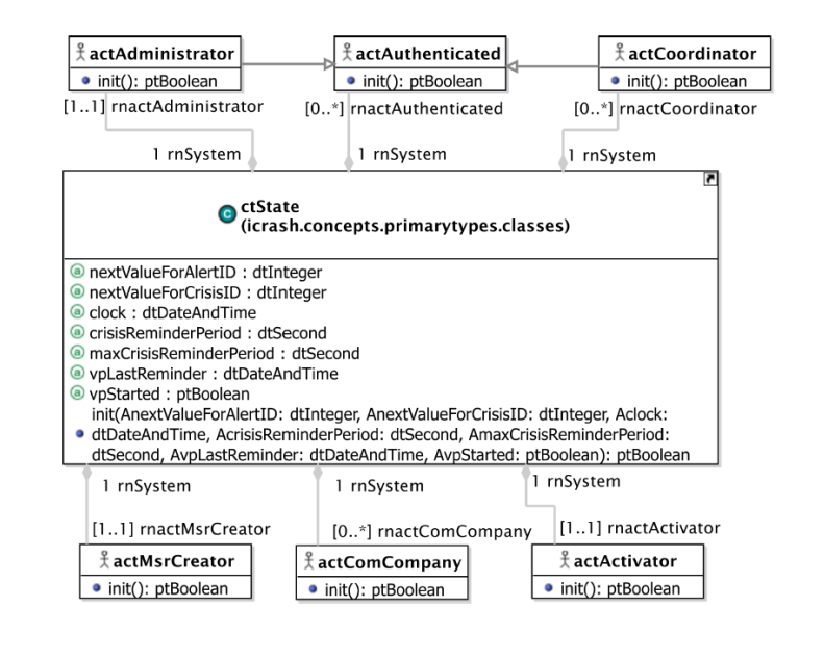
\includegraphics[width=0.9\textwidth]{./images/env_model.eps}
\end{center}
\caption{Environment Model}
\end{figure}
